\section{Reto de extensión}
\label{sec:p2-reto}

El instructivo propone refactorizar \texttt{CalculadoraImpl} para registrar cada invocación en una bitácora persistente, introducir un segundo objeto remoto \texttt{BitacoraRemota} que permita al cliente consultar el historial de operaciones, y configurar RMI sobre SSL/TLS mediante una \texttt{RMIClientSocketFactory} y una \texttt{RMIServerSocketFactory} que utilicen un certificado autofirmado, documentando el \emph{handshake} observado con \texttt{tcpdump} o Wireshark. Las tres partes se implementaron directamente en la Sección de desarrollo de este capítulo; aquí se documentan las dos simplificaciones deliberadas y la evidencia específica de la extensión.

\subsection*{Simplificación 1: bitácora en archivo de texto en vez de PostgreSQL/SQLite}

El contenedor de esta práctica no tiene salida a Internet para descargar un controlador JDBC ni el paquete de un motor de base de datos adicional. Para no desviar el alcance de la práctica hacia la administración de un sistema de gestión de bases de datos, la bitácora se implementó como un archivo de texto plano de solo anexado (\texttt{/tmp/bitacora.log}), protegido con \texttt{synchronized} para escrituras concurrentes. Cumple el mismo rol didáctico —un segundo objeto remoto con estado persistente entre invocaciones— sin introducir una dependencia externa no disponible en el entorno.

\subsection*{Simplificación 2: certificado y \emph{truststore} compartidos}

Se generó un único almacén de llaves (\texttt{certs.jks}) con \texttt{keytool -genkeypair} durante la construcción de la imagen, y ese mismo archivo se referenció como \emph{truststore} tanto en el servidor como en el cliente (\texttt{javax.net.ssl.trustStore}). En un despliegue de producción el certificado público se exportaría a un \emph{truststore} independiente distribuido solo al cliente; para los fines de esta práctica de laboratorio, compartir el almacén es suficiente para demostrar el cifrado de la capa de transporte sin la sobrecarga operativa de gestionar dos almacenes distintos.

\begin{lstlisting}[language=bash]
$ keytool -genkeypair -alias rmiserver -keyalg RSA -keysize 2048 \
    -dname "CN=esimecu-vm, OU=ESIME Culhuacan, O=IPN, L=CDMX, C=MX" \
    -validity 365 -keystore /rmi-lab/certs.jks -storepass changeit -keypass changeit
\end{lstlisting}

\subsection*{Evidencia de la bitácora persistente}

\begin{lstlisting}
$ cat /tmp/bitacora.log
2026-07-20T00:49:47.241 | sumar(3.0, 4.0) = 7.0
2026-07-20T00:49:47.255 | restar(10.0, 6.0) = 4.0
2026-07-20T00:49:47.258 | multiplicar(7.0, 8.0) = 56.0
2026-07-20T00:49:47.268 | dividir(5.0, 0.0) -> ERROR división entre cero
2026-07-20T00:50:19.015 | sumar(3.0, 4.0) = 7.0
2026-07-20T00:50:19.023 | restar(10.0, 6.0) = 4.0
2026-07-20T00:50:19.024 | multiplicar(7.0, 8.0) = 56.0
2026-07-20T00:50:19.026 | dividir(5.0, 0.0) -> ERROR división entre cero
\end{lstlisting}

\begin{figure}[H]
\centering
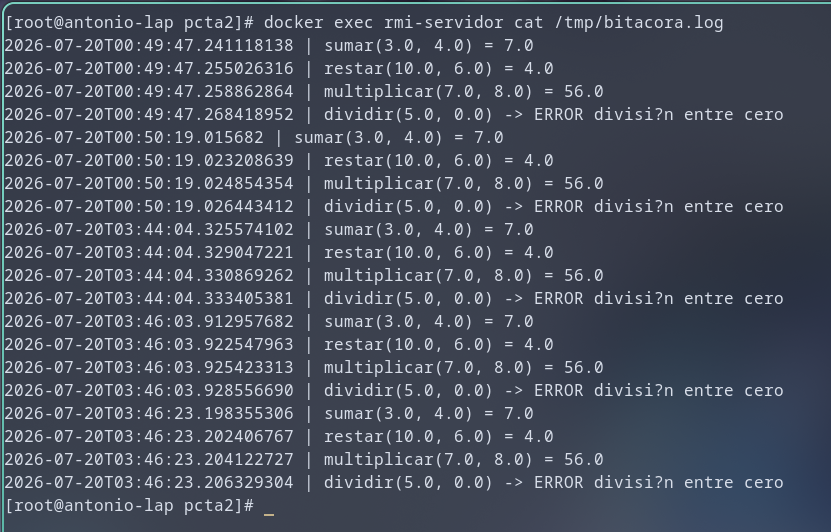
\includegraphics[width=0.85\linewidth]{../src/ss/3.6.png}
\caption{Contenido de \texttt{/tmp/bitacora.log} en el contenedor \texttt{rmi-servidor}: registro persistente de todas las corridas del cliente.}
\label{fig:p2-reto-bitacora}
\end{figure}

La Figura~\ref{fig:p2-reto-bitacora} muestra el archivo con las invocaciones de \emph{cuatro} ejecuciones distintas del cliente, identificables por sus marcas de tiempo (00:49, 00:50, 03:44 y 03:46). Cada bloque repite el mismo patrón de cuatro operaciones, incluida la división entre cero registrada como error. Que las entradas antiguas sobrevivan a cada nueva corrida del cliente confirma la propiedad que el reto busca demostrar: el objeto remoto mantiene estado durable en el servidor, independiente del ciclo de vida de los clientes que lo invocan. Obsérvese además que el registro lo escribe \texttt{CalculadoraImpl} invocando a \texttt{BitacoraRemota} —una llamada entre objetos remotos del mismo proceso—, patrón que en un sistema real correspondería a la composición de microservicios.

\subsection*{Evidencia del handshake TLS}

El análisis de tráfico de la Sección de desarrollo (Figura~\ref{fig:p2-tcpdump}) ya documenta el fragmento hexadecimal del \emph{ClientHello} capturado en el puerto efímero exportado con \texttt{SslRMIServerSocketFactory}, distinto del puerto 1099 del \texttt{rmiregistry} (que permanece en JRMP sin cifrar, ya que el registro en sí no se exportó con fábricas SSL). Esa distinción —registro en claro, invocación de objetos cifrada— es intencional: ilustra que la extensión con TLS protege la comunicación con la lógica de negocio, no el servicio de nombres, que en un despliegue real se restringiría por firewall en vez de por cifrado.
